
\subsubsection{Space plasma physics}
\index{Vogt, Joachim}
\label{GeoAstro:Vogt}

\paragraph{Research Team}
Dr. Joachim Vogt (Professor), Dr. Bertalan Zieger,
Dr. Matthias Hoeft (since August 2006)\\

The structure and dynamics of near-Earth space are controlled
by the interaction of the geomagnetic field with the stream
of solar particles called the solar wind.  This interaction
leads to the formation of a magnetic cavity in space that is
commonly referred to as the Earth's magnetosphere.  The highly variable
solar wind causes magnetospheric dynamics on short timescales of hours
to days which leads to space weather phenomena like geomagnetic
storms, auroral emissions, failures of communication satellites, and
electrical power disruptions on the ground.  On geological timescales,
variations of the geomagnetic core field are expected to have
a strong effect on the magnetospheric structure and on the behaviour of
energetic particles in near-Earth space.  At IUB, magnetosphere formation
and other space plasma processes are studied using large-scale
magnetohydrodynamic (MHD) simulations, plasma theory, and data
from spacecraft.


\paragraph{Highlights}

The DFG funded project \emph{Studies of paleomagnetospheric processes\/}
dealt with the magnetosphere during geomagnetic polarity transition periods.
In a paper published in the Journal of Geophysical Research, MHD simulation
results were compared with an empirical model for the size and the shape
of the magnetospheric boundary layer (magnetopause).  Very good agreement
was found within the validity range of the empirical model.  Outside this
range our MHD simulations offer a more complete description of the
magnetopause shape and size in terms of solar wind parameters and the
geomagnetic dipole moment.  The empirical model could be generalized
beyond the former validity range.
In a second study, the distribution of energetic particles in the
paleomagnetosphere was investigated by analytical means.  Since our
collaborators at the universities in Bremen and Osnabr{\"u}ck use our
results as input to model the chemistry of the middle atmosphere in
response to solar energetic particle events, we were particularly
interested in the polar cap region that is most affected by such
particle events.  Our results indicate that with decreasing dipole
moment and increasing quadrupole contribution, this region can extend
down to latitudes as low as 40 degrees.
More complex magnetic field configurations are modelled using
MHD simulation results and field line tracing schemes.
Figure~\ref{fig:Vogt_2006_Fig} illustrates how the open field line
region may look like during a geomagnetic polarity transition with a
highly non-axisymmetric core field.  An invited paper on the results
of this project and on the work of our collaborators within the
DFG Priority Programme SPP 1097 was presented at a DFG Colloquium.

\begin{figure}[ht]
  \begin{center}
    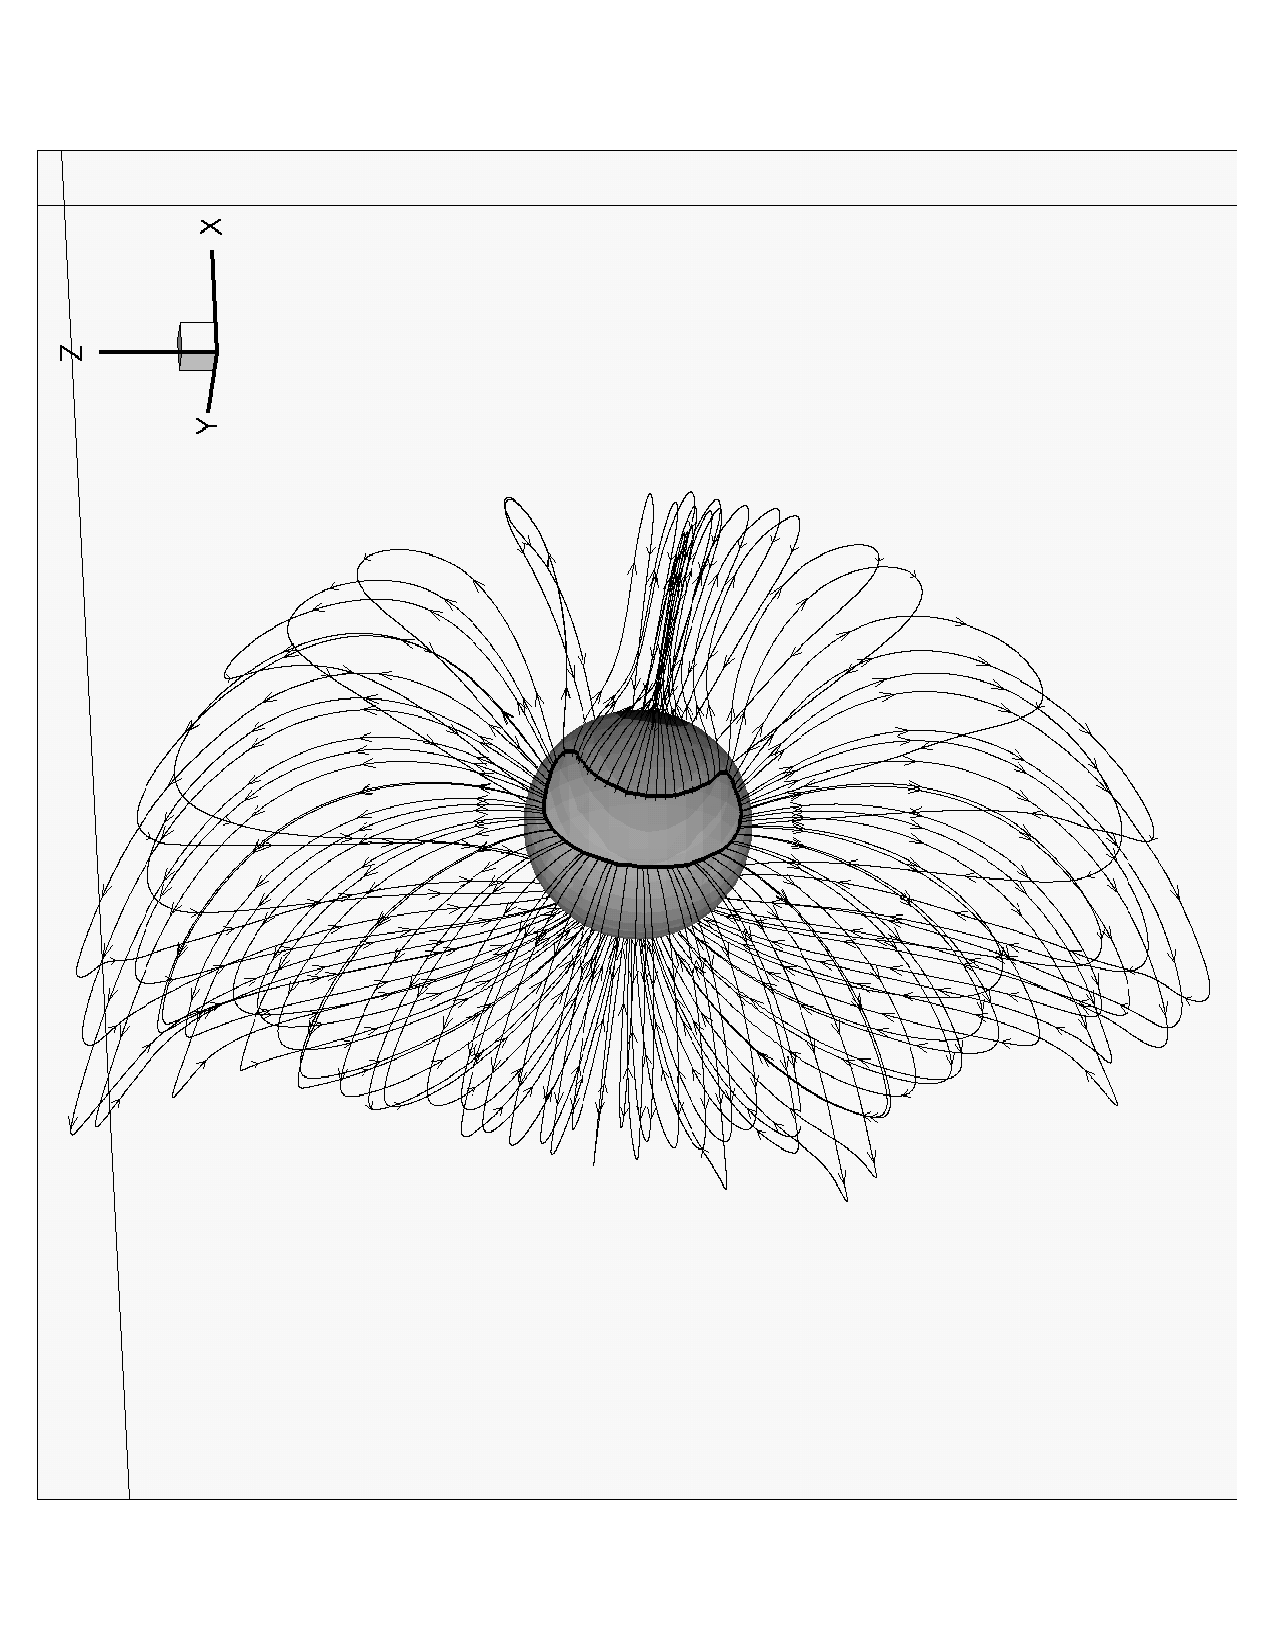
\includegraphics[height=\hsize, angle=270]{Vogt/Vogt_2006_Fig}
    \mycaption{Closed magnetic field lines in a simulated paleomagnetosphere.
               The region in the center is penetrated by open field lines
               (not shown) and thus accessible by low-rigidity particles
               from solar energetic particle events.  Figure produced
               by Bertalan Zieger.}
    \label{fig:Vogt_2006_Fig}
  \end{center}
\end{figure}

In a second DFG funded space plasma project (jointly with Prof. Marcus
Br{\"u}ggen and Dr. Matthias Hoeft), we are planning to model radio emissions
of coronal mass ejections which happen on time scales like hours or days,
and lead to space weather phenomena like geomagnetic storms and substorms.
The project started in August 2006.

Supervised jointly by faculty from marine geosciences (Prof. Laurenz
Thomsen) and space physics (Prof. Joachim Vogt), the GeoAstro student team
\emph{Neptunas\/} participated in ESA's Student Parabolic Flight Campaign
2006.  During two parabolic flights on the Zero-G Airbus A-300,
four 3rd-year students Simona Balan, Matteo Kausch, Eva St\"ueken, and
Wilken-Jon von Appen studied the influence of microcravity on the
photosynthetic yield of microalgae.  The students received support also
from industry (OHB System, Bluebiotech, Heinz Walz GmbH).



\paragraph{Organization}

\begin{enumerate}
\item
COSPAR Capacity Building Workshop to be held in June 2007, Sinaia, Romania
(jointly organized with Prof. Peter Willmore, University of Birmingham,
Prof. Thierry Dudok de Wit, CNRS Orleans, Dr. Octav Marghitu, MPE Garching
and ISS Magurele, Dr. Marius Echim, BIRA Bruxelles and ISS Magurele).
Sponsored by COSPAR, ROSA, and other space organisations.
\item
Successful WAP proposal to renew the computational infrastructure of the
CLAMV Teaching Lab (jointly with Prof. Martin Zacharias, Dr. Achim Gelessus,
and Dr. Heinrich Stamerjohanns).
\end{enumerate}


\paragraph{Collaborations}\noindent

Regional:
\begin{enumerate}
\item
{\sl Technische Universit{\"a}t Braunschweig}\\
Prof. Karl-Heinz Glassmeier
\item
{\sl International University Bremen}\\ Prof. Marcus Br{\"u}ggen,
Prof. Laurenz Thomsen, Prof. Vikram Unnithan
\item
{\sl Universit{\"a}t Osnabr{\"u}ck}\\
Prof. May-Britt Kallenrode
\item
{\sl Universit{\"a}t Bremen}\\
Dr. Miriam Sinnhuber
\item
{\sl OHB-System, Bremen}\\ Dr. Klaus Slenzka
\end{enumerate}

National:
\begin{enumerate}
\item
{\sl Ruhr-Universit{\"a}t Bochum}\\
Prof. Reinhard Schlickeiser, Priv.-Doz. Dr. Horst Fichtner
\end{enumerate}

International:
\begin{enumerate}
\item
{\sl University of Michigan, Ann Arbor, USA}\\
Prof. Tamas Gombosi, Dr. Ward Manchester
\item
{\sl ASTRON, The Netherlands}\\ Dr. Michiel van Haarlem
\end{enumerate}


\paragraph{Grants}

\begin{enumerate}
\item
Funded by DFG, \emph{Studies of paleomagnetospheric processes}
(October 2004 - December 2006)
\item
Funded by DFG, \emph{The CME source region in LOFAR related
simulations} (January 2006 - March 2008)
\end{enumerate}

\paragraph{Other Support Grants}
\begin{enumerate}
\item Support from the European Space Agency (ESA) and from
industry (OHB System, Bluebiotech, Heinz Walz GmbH) for the GeoAstro
student team \emph{Neptunas\/} to participate in the \emph{ESA
Student Parabolic Flight Campaign 2006\/}.
\end{enumerate}
\nocite{vogt:terra-nostra-vogt-etal-2006}
\nocite{vogt:asr-zieger-etal-2006}
\nocite{vogt:jgr-zieger-etal-2006}
